% SPDX-FileCopyrightText: Copyright (c) 2023 Yegor Bugayenko
% SPDX-License-Identifier: MIT

\documentclass{article}
\usepackage{../../lecture-notes/notes}

\graphicspath{{../../faces/}}

\newcommand*{\thetitle}{Open Source Kung-Fu}
\newcommand*{\thesubtitle}{Nine Levels of It}
\newcommand*{\theauthor}{Yegor Bugayenko}

\newcounter{level}
\newcommand\level[1]{\stepcounter{level}\plush{\pptChapter[L\thelevel]{#1}}}

\begin{document}

\pptLeft{%
  \includegraphics[height=3em]{kungfu.pdf}\\
  
\includegraphics[height=1.4em]{neimark-logo.png}\\[.6em]
  October 18th, 2024}
\pptRight{@yegor256}

\plush{
  \begin{pptMiddle}
    \includegraphics[height=5em]{kungfu.pdf}
    \pptTitle{\thetitle}{\thesubtitle}\par
    {\scshape \theauthor}
    \newline
    {\small Zerocracy\par}
  \end{pptMiddle}
}

\lnPitch{
  \begin{tabular}{lr}
    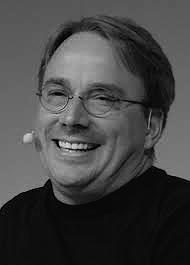
\includegraphics[height=6em]{linus-torvalds.jpg}
    &
    
\includegraphics[height=6em]{mauro-carvalho-chehab.jpg} \\
    \multicolumn{2}{l}{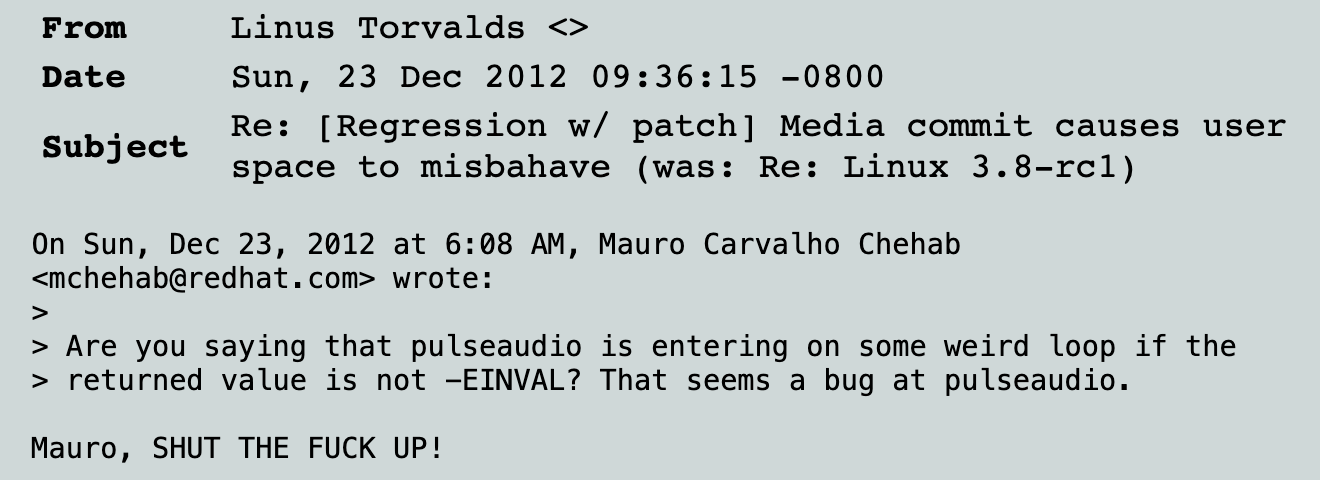
\includegraphics[width=.7\linewidth]{linus-email.png}}
  \end{tabular}}

\lnQuote
  [\nospell{Isabella Ferreira}]
  {isabella-ferreira}
  {We conducted a qualitative analysis on 1,545 emails from the Linux Kernel Mailing List that were associated with rejected changes. We found that \ul{more than half} (67\%) of the non-technical emails included uncivil features. Particularly, \textcolor{orange}{frustration}, \textcolor{orange}{name calling}, and \textcolor{orange}{impatience} are the most frequent features in uncivil emails. }
  {ferreira2021shut}

\level{You've got your own GitHub account}

\lnQuote
  [\nospell{Kristine Nowak}]
  {kristine-nowak}
  {Avatars that were more \ul{anthropomorphic} were perceived to be more \ul{attractive} and \ul{credible}. The strongest predictor of these variables, however, was the degree of masculinity or femininity (lack of androgyny) of an avatar.}
  {nowak2005influence}

\lnPitch{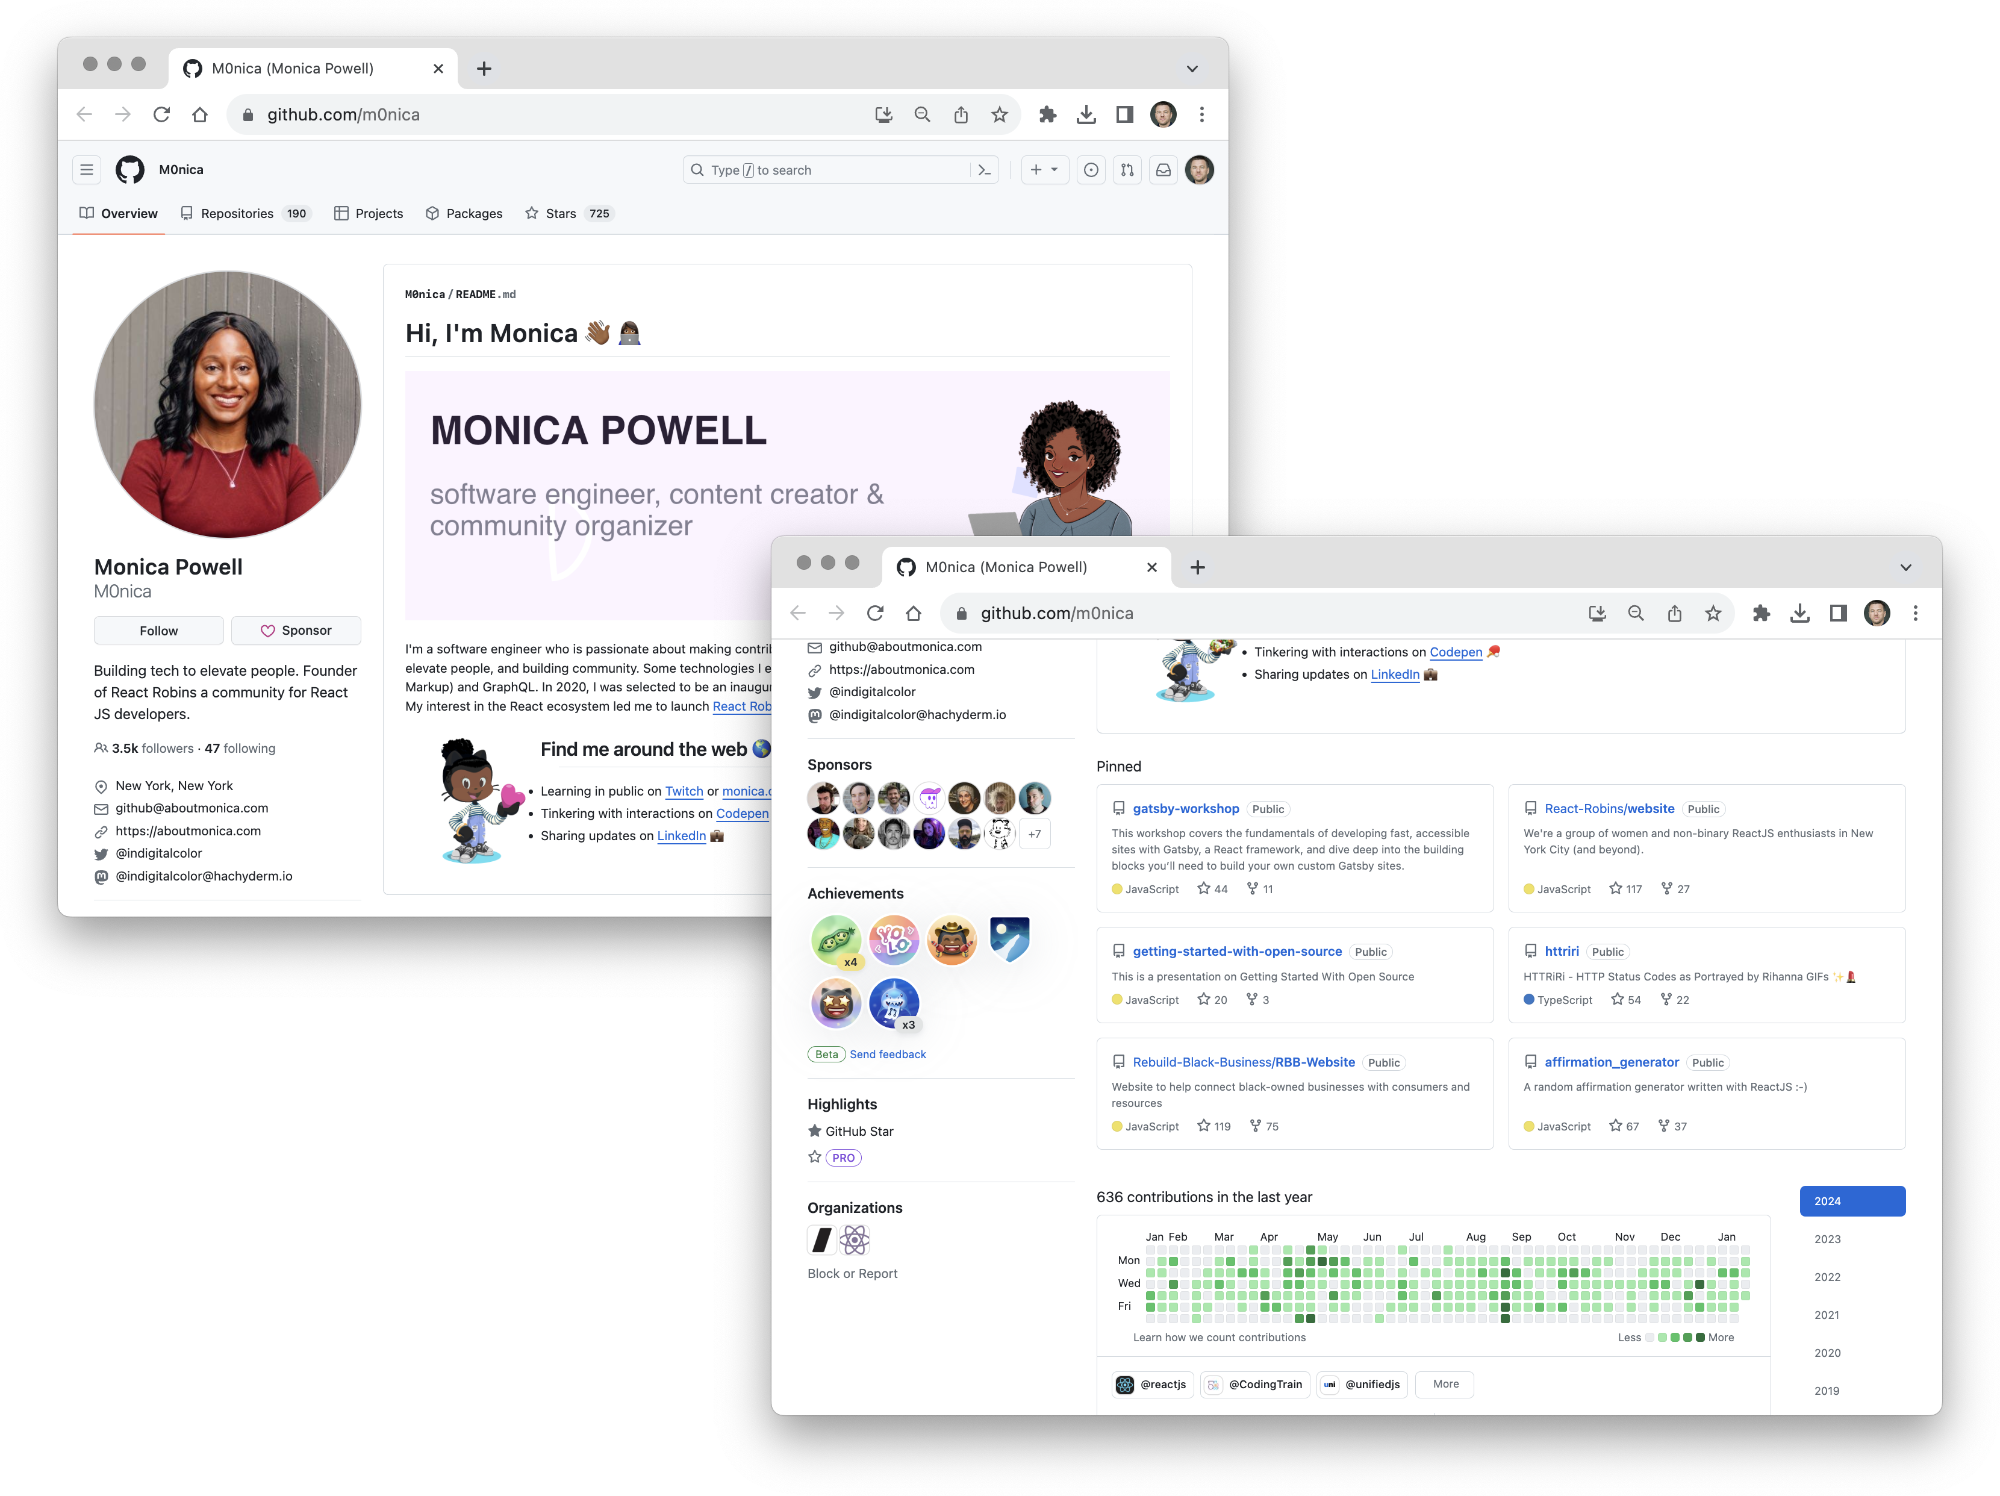
\includegraphics[width=.75\linewidth]{monica.png}}

\level{Your pull request has been merged}

\lnQuote
  [\nospell{\nospell{Bram Adams}}]
  {bram-adams}
  {We found that \ul{33\%} of the patches makes it into a Linux release, and that most of them need \ul{3 to 6 months} for this.}
  {jiang2013will}

\lnQuote
  [\nospell{Jacek Czerwonka}]
  {jacek-czerwonka}
  {Only about 15\% of comments provided by reviewers indicate a possible defect, much less a blocking defect. Rather, it is feedback related to the long-term code \ul{maintainability} that comprises a much larger portion of comments provided by reviewers; at least 50\% of all.}
  {czerwonka2015code}

\lnQuote
  [\nospell{Caitlin Sadowski}]
  {caitlin-sadowski}
  {A correlation between \ul{change size} and \ul{review quality} is acknowledged by Google and developers are strongly encouraged to make small, incremental changes (with the exception of large deletions and automated refactoring).}
  {sadowski2018modern}

\lnQuote
  [\nospell{Carolyn D. Egelman}]
  {carolyn-egelman}
  {Google categorizes CRs into specific sizes, these sizes are indicated as part of the code review tool and in the notification to the reviewer of the code change... The general advice is to \ul{split} change requests for \ul{easier} and \ul{quicker} reviews when possible.}
  {egelman2020predicting}

\lnQuote
  [\nospell{Marco Ortu}]
  {marco-ortu}
  {Our results show that \ul{valence} (expressed in comments received and posted by a reporter) and \ul{joy} expressed in the comments written by a reporter are linked to a \ul{higher likelihood} of issues to be merged. On the contrary, sadness, anger, and arousal expressed in the comments written by a reporter, and anger, arousal, and dominance expressed in the comments received by a reporter, are linked to a lower likelihood of a pull request to be merged.}
  {ortu2020you}

\lnQuote
  [\nospell{Valentina Lenarduzzi}]
  {valentina-lenarduzzi}
  {Unexpectedly, quality \ul{flaws} measured by PMD turned out not to affect the acceptance of a pull request at all. As suggested by other works, other factors such as the \ul{reputation} of the maintainer and the \ul{importance} of the delivered feature might be more important than other qualities in terms of pull request acceptance.}
  {lenarduzzi2021does}

\level{You've released a package}

\lnQuote
  [\nospell{Michael Nygard}]
  {michael-nygard}
  {Releases should be about as big an event as getting a \ul{haircut}. There's an added benefit of frequent releases: it forces you to get really good at doing releases and deployments.}
  {nygard2007release}

\lnQuote
  [\nospell{Jez Humble}]
  {jez-humble}
  {Over time, deployments should tend towards being fully automated. There should be \ul{two tasks} for a human being to perform to deploy software into a development, test, or production environment: to pick the version and environment and to press the `deploy' button.}
  {humble2010continuous}

\level{You've received a pull request}

\lnQuote
  [Simon Weber]
  {simon-weber}
  {Upon investigation, popular projects were found to have larger READMEs (median 2 kilobytes vs. 500 bytes). Also, 95\% of popular projects have nonempty READMEs, compared to only 65\% of unpopular projects.}
  {weber2014makes}

\lnQuote
  [\nospell{Asher Trockman}]
  {asher-trockman}
  {We find that non-trivial \ul{badges}, which display the build status, test coverage, and up-to-dateness of dependencies, are mostly reliable signals, correlating with more tests, better pull requests, and fresher dependencies.}
  {trockman2018adding}

\lnQuote
  [\nospell{Shaowei Wang}]
  {shaowei-wang}
  {The frequency/number of readme \ul{updates} and the number of \ul{lists} and \ul{links} positively correlate with the likelihood of a repository being popular.}
  {wang2023study}

\level{Your repository's been taken over}

\plush{
  \begin{multicols}{2}
  \pptPic{.9}{micromap.png}
  \par\columnbreak\par
  \pptPic{.9}{benchmark.png}
  \end{multicols}
  Thanks to \href{https://github.com/zefick}{@Zefick}!}

\level{Your repository's got 100 bugs}

\lnQuote
  [\nospell{Myers, Glenford J.}]
  {glenford-myers}
  {You cannot test a program to guarantee that it is error free... It is impractical, often impossible, to find \ul{all} the errors in a program.}
  {myers2012art}

\lnQuote
  [\nospell{Reis Christian}]
  {reis-christian}
  {Though it commonly has a prejorative connotation, in the Mozilla Project the term \textbf{bug} is used to refer to any field request for modification in the software, be it an \ul{actual} defect, an enhancement, or a change in functionality. (``bug-driven development'')}
  {reis2002overview}

\lnPitch{\pptBanner{Repositories With a Lot of Bugs (9 Feb 2024)}
  {\small\begin{tabular}{lr}
  \toprule
  Github Repository & Bugs \\
  \midrule
  \href{https://bugzilla.mozilla.org/}{mozilla} & 1,8M+ \\
  \href{https://gitlab.com/gitlab-org/gitlab/-/issues}{\texttt{gitlab-org/gitlab}} & 172,462 \\
  \href{https://github.com/flutter/flutter}{\texttt{flutter/flutter}} & 79,386 \\
  \href{https://github.com/kubernetes/kubernetes}{\texttt{kubernetes/kubernetes}} & 42,627 \\
  \href{https://github.com/tensorflow/tensorflow}{\texttt{tensorflow/tensorflow}} & 36,776 \\
  \href{https://github.com/moby/moby}{\texttt{moby/moby}} & 19,367 \\
  \bottomrule
  \end{tabular}}\par
  All repositories are open source.}

\level{Google's offered you a retainer}

\plush{\pptPic{.9}{github-email.png}}

\level{GitHub's offered you large runners}

\plush{
  \begin{multicols}{2}
  \pptPic{.9}{alexander.png}\par
  Watch the interview \href{https://www.youtube.com/watch?v=xMGNlUZQ-6w}{on YouTube}.\par
  \qrcode[height=4em]{https://www.youtube.com/watch?v=xMGNlUZQ-6w}
  \par\columnbreak\par
  \textcolor{orange}{Alexander Medvednikov}, the creator of the \href{https://vlang.io/}{V programming language},
  in the interview mentioned that GitHub offers his project free access
  to larger CI/CD resources (aka ``\textcolor{orange}{large runners}'').\par
  
\includegraphics[width=3em]{v-logo.png}\par
  \href{https://vlang.io/}{www.vlang.io}
  \end{multicols}}

\level{Sponsors've given you \$100K/year}

\plush{
  \begin{multicols}{2}
  \pptPic{.9}{sponsors-1.png}\par
  Read the story of \href{https://github.com/calebporzio}{\textcolor{orange}{Caleb Porzio}},
  and \href{https://github.com/readme/stories/caleb-porzio}{this one} too.\par
  He is the creator of \href{https://github.com/livewire/livewire}{LiveWire} (22K\(\star\))
  and \href{https://github.com/alpinejs/alpine}{AlpineJS} (28K\(\star\)).
  \par\columnbreak\par
  
\includegraphics[width=\linewidth]{caleb-porzio.jpg}\par
  \pptPic{.9}{sponsors-2.png}
  \end{multicols}}

\plush{\pptChapter[Next]{What's next?}}

\plush{
  \begin{multicols}{2}
  \pptBanner{1)~Subscribe:}\par
  \qrcode[height=6em]{https://t.me/yegor256news}\par
  \href{https://t.me/yegor256news}{\texttt{@yegor256news}}\par
  \pptBanner{3)~Join:}\par
  Text me if you need a topic for your open source project or ready to join one of ours.
  \par\columnbreak\par
  \pptBanner{2)~Watch:}\par
  \qrcode[height=6em]{https://www.youtube.com/playlist?list=PLaIsQH4uc08zjutyoBOtoa6fnxzrCQK2Q}\par
  ``Open Source Best Practices'' Course of Eight Lectures for Innopolis University:
  \href{https://www.youtube.com/playlist?list=PLaIsQH4uc08zjutyoBOtoa6fnxzrCQK2Q}{\texttt{PlayList}}
  \end{multicols}}

\end{document}
